%%%%%%%  Referencias %%%%%%
%https://es.overleaf.com/learn/latex/Code_listing
%
%%%%%%

\documentclass[12pt]{article}

\title{Sistema concurrente CARDIAC}
\author{Martín Osvaldo Santos Soto}
\date{\today}


%Packages
\usepackage[letterpaper,top=2cm,bottom=2cm,left=2cm,right=2cm]{geometry}
\usepackage[utf8]{inputenc}
\usepackage[spanish, activeacute]{babel}

%Subfiguras
\usepackage{caption}
\usepackage{subcaption}

% Para referencias 
\usepackage{hyperref}
\usepackage{apacite}
\usepackage{url}

\usepackage{graphicx} 

\begin{document}
	\maketitle

    %¿Que es cardiac concurrente? opción de titulo inicial y breve descripción que conteste a las siguientes preguntas:
    %¿Por que? ¿Por que no es suficiente CARDIAC?  ¿Que necesita? ¿Por que necesita el bootloader?
	
	\section{ Arranque del sistema} % Dejar esta parte como subsección
 	 
 	 Para lograr la concurrencia se ha necesitado cambiar la arquitectura de CARDIAC, los cambios han sido menores pero significativos
	 para lograr el objetivo. Primero debemos definir un ``programa'' que será central, el \textit{bootloader}, basado
	 completamente en el mecanismo de \textit{bootstraping} que presenta la página de CARDIAC \cite{noauthor_cardiac_nodate}. El \textit{bootstraping} es un 
	 mecanismo que todas las computadoras tienen hoy en día en un nivel mucho más complejo que el que se puede lograr con CARDIAC, sin
	 embargo con CARDIAC se puede lograr el punto básico, crear un mecanismo de arranque inicial para la computadora, de tal forma
	 que la computadora con solo instrucciones del usuario pueda recibir programas y ejecutarlas. 
	 
	 La idea del \textit{bootstraping} se explicará para el sistema CARDIAC normal pero es fácilmente extensible para el modificado
	 que se presentará. Cuando se inicia CARDIAC en la dirección $00$ ya se encuentra la instrucción $01$, por lo que te pedirá
	 que ingreses una entrada que se guardará en la dirección $01$, lo que se debe hacer es ingresar la instrucción $02$, así
	 que el \textit{program counter} se moverá hacia la dirección $01$ y pedirá otra entrada a guardar en la dirección $02$, ahora
	 ingresas $800$, así cuando se mueva el contador hacia $02$ se encontrará con que tiene que saltar hacia el inicio de nuevo. De
	 esta forma se ha creado un \textit{loop} en el cual el usuario, siguiendo unas reglas simples, puede escribir su programa
	 y ejecutarlo, sino estuviera este programa de arranque el usuario tendría que colocar su programa en CARDIAC de alguna forma
	 que externa al propio funcionamiento del sistema. Las reglas son las siguientes, como se ha regresado a la dirección
	 inicial el programa pedirá que el usuario ingrese un valor que se guardará en $01$, el usuario debe ingresar la dirección que
	 quiere que sea la inicial para su futuro programa con el \textit{op-code} $0$, por que el contador leerá justamente esa instrucción
	 en el siguiente paso, por lo que una vez hecho eso el usuario ingresará la primera instrucción de su programa, después llegará a la
	 dirección $02$ y saltará al inicio para repetir el proceso, esto lo hará el usuario hasta que haya guardado la última instrucción
	 de su programa en la dirección correspondiente, para terminar solo tendrá que escribir una instrucción más, la $8xx$, donde
	 $xx$ es la dirección de inicio del programa que acaba de ingresar el usuario. Así el usuario ingresando \textbf{pares} de 
	 instrucciones de la forma:
	
	 \begin{verbatim}
		 010
		 111
		 ...
		 
		 ...		 
		 020
		 900
		 810
	 \end{verbatim}
	
	cargará su programa en iniciando en la dirección $10$ y terminando en la dirección $20$ con la instrucción final del programa pero
	no del usuario por que el usuario aún saltará hacia el inicio de su programa con una instrucción que ya no va en forma de par. En
	este punto se puede preguntar como regresará al \textit{loop} de inicio una vez fuera, pero ese es un detalle que se solucionará con
	el administrador de tareas, ya que este \textit{bootstraping} esta creado para ser el \textit{bootloader} en la implementación concurrente
	de CARDIAC que complementa al \textbf{sistema operativo} que esta tendrá, así que se puede considerar a esta forma de
	agregar programas como una versión incompleta y que no será la definitiva
	, en la página de \cite{noauthor_cardiac_nodate} se detalla una implementación que no contempla un sistema operativo por si se quiere revisar.
	

    % Maquina concurrente
    % Nuestra maquina esta diseñada para funcionar solo con sistema operativo, ¿por que no funcionaria sin el?¿Por que es necesario?
	\section{CARDIAC v2}
	
	En esta sección se describirán las características nuevas que tendrá la arquitectura para lograr la concurrencia. Primero vayamos a
	las instrucciones, estas se mantendrán sin cambios a excepción de la instrucción \textbf{HALT} o $9000$ para terminar un programa que
	sufrirá una ligera mejora, esta terminará un programa como siempre pero a su vez saltará a una dirección especial, a tal
	dirección la llamaremos \textbf{B}, en tal dirección se continuará la ejecución, después mencionaremos que es lo que se hará a partir
	de ahí. La otra cuestión con las instrucciones es que ya no será una arquitectura para direcciones del 1 al 100, sino para
	que sea del 1 al 1000, y de hecho la arquitectura esta preparada para soportar una cantidad de memoria de cualquier múltiplo de 10 mayor
	a 100, pero no sirve de mucho cuando la intención es mostrarle al estudiante lo que pasa en ahí si la memoria tiene
	100,000 celdas; como la arquitectura ahora es para más direcciones es natural pensar que las instrucciones deben cambiar, pero no es
	así, las instrucciones seguirán siendo el primer dígito(a la izquierda) representa al \textbf{op-code} y los otros
	tres dígitos representan una dirección, el caso especial de \textbf{SHIFT} esta considerado y aquí si hay un pequeño detalle,
	el primer dígito será para el \textbf{op-code} y los dos últimos para los movimientos a izquierda y derecha tal como
	se describen en la arquitectura original, el dígito que esta en medio(en la segunda posición de izquierda a derecha) no
	se toma en cuenta.
	% En la tabla tal podemos ver las instrucciones
	% Insertar tabla de comando de ejemplo
	
	Una vez conocidas las instrucciones con las que seremos capaces de programar hay que saber como funciona esta computadora, podemos
	considerar que sigue todas las directrices que su antecesora pero con algunas funciones extra.
	
	\begin{itemize}
		\item Saltos del contador de programa(Program counter):  
			El contador de programa para permitirle al sistema operativo ser el que controle realmente que se ejecutará saltará
			cada \textit{C} ciclos(si su bandera de salto esta activa) desde el punto en donde este hacia la dirección \textbf{alfa}.
			La cantidad \textit{C} será establecida cuando se cree la maquina y puede tomar cualquier valor mayor a cero, mientras
			que la dirección \textbf{alfa} será una `` entrada'' al sistema operativo, esto último ya se detallará más adelante
			cuando hablemos de lleno sobre el sistema operativo.
		
		\item Bandera de salto automático del contador de programa: 
			Esta bandera estará en la dirección $003$ y es la que servirá para que el contador de programa salte en automático cada $C$
			ciclos hacia \textbf{alfa} o si por el contrario el contador de programa debe seguir su funcionamiento habitual avanzando
			avanzando de uno en uno por cada dirección y saltando solo cuando una instrucción se lo indica. Para lograr este accionar
			la dirección $003$ tendrá conectado un bus especial de color rosa que conecta directamente con el contador de programa, si
			la bandera tiene el número $0$ no se permitirán los saltos automáticos, en cambio si tiene el valor $1$ cada $c$ ciclos el
			contador de programa saltará hacia \textbf{alfa}.
			
		\item Guardado automático de contador de programa:
			Esto entrará en función únicamente si la bandera de $003$ esta posicionada en $1$ y por ende permitir saltos automáticos,
			justo antes de hacer el salto un bus especial de color plata conectado directamente a la dirección especial \textbf{e} donde
			guardará el valor que tiene el contador de programa en ese momento y justo después de eso saltará el contador de programa.
			% ¿Podemos decir que en este proceso se pierde un ciclo?
			
	\end{itemize}
	
	Las modificaciones son lo más imperceptibles que se puede para afectar muy poco a la arquitectura original, demostrando
	lo robusta que es la arquitectura principal que en principio puede parecer bastante simple.
	
	Ahora si ya tenemos todos los ingredientes para la concurrencia, solo falta alguien que los controle y saque el mayor provecho
	posible de ellos, \textbf{el sistema operativo}.
	
	
	\section{ Sistema operativo}
	%SO sistema operativo
	%pc contador de programa
	%acc acumulador
	
	El sistema operativo es el encargado de administrar los recursos de la maquina y esta dentro de la memoria de la misma, por lo
	que se le puede considerar como un programa muy especial. El sistema operativo que usará CARDIAC realizará tres 4 funciones
	principales:
	
	\begin{itemize}
		\item Actualizar proceso
		\item Borrar proceso
		\item Agregar proceso
		\item Lanzar proceso
	\end{itemize}
	
	Como habrán notado usamos la palabra \textit{proceso} y no la de programa, y es que cuando un programa se esta ejecutando
	se vuelve más que un simple programa, pero eso se explicará un poco más adelante, por ahora lo importante es notar que
	el sistema operativo necesita varias cosas para funcionar: recibir los valores correctos, un lugar donde
	guardar estos ``extraños'' procesos, y uno donde guardar variables que le sean de utilidad. Para solucionar estos
	problemas y que sea claro para el lector como se funciona este sistema operativo
	hemos decidido dividir en 4 regiones de memoria las celdas que ocupará el
	sistema operativo, aunque solo una de ellas llevará a cabo las operaciones mencionadas en la lista anterior. Las regiones
	son:
	
	\begin{itemize}
		\item Sistema operativo central: Es como tal la región que realiza la operaciones mencionadas en la lista anterior.
		\item Preámbulo o exordio: Esta se encarga de que los valores que solicita el sistema operativo lleguen con el
		formato y detalles que este exige.
		\item Zona de procesos: Aquí se almacenará toda la información concerniente a los procesos.
		\item Variables del sistema: En esta se encuentran diversas variables y algunas constantes que le servirán al sistema
		para su funcionamiento.
	\end{itemize}
	
	
	% Explicar la nomenclatura antes de entrar aquí
	\subsection{Zona de procesos}
	
	Vamos a detallar lo que hay exactamente en cada una de estas regiones, empezando por la \textbf{Zona de proceso}, pero
	hay que definir primero lo que es un proceso. Antes mencione que era algo más que un programa, lo definir muy a la ligera
	en ese punto, un proceso es un conjunto de elementos asociados a la ejecución de un programa, es por ello que se
	suele decir que un proceso es un programa en ejecución. Los componentes que tendrán nuestros proceso básicos son un
	\textbf{id} que permita identificarlos de manera única, el contador de programa o \textbf{gpc} por el hecho de ser el contador
	de programa guardado, y el acumulador o \textbf{gacc} por ser el acumulador guardado. Estos tres componentes logran identificar
	de manera única la ejecución de un programa en cualquier instante dentro de sus ciclos de vida, es gracias a estos que
	podemos hacer programación concurrente, pues cada vez que saltamos a la mitad de un programa hacia el sistema operativo 
	el programa que se estaba ejecutando ya no estaba en el inicio estaba en cualquier dirección posible y tal vez ya
	habría hecho alguna operación por lo que el acumulador también tenia un valor propio del programa en ese instante de la ejecución,
	para poder saltar y regresar al mismo instante con el mismo acumulador es necesario guardar esos valores, y es por eso que los
	procesos nos permiten la ejecución concurrente de instrucciones. 
	
	En la imagen \ref{fig:zprocesos} se ve la representación
	de esta en un conjunto de direcciones especiales iniciadas con $p0$ que representan una sucesión de direcciones
	que pueden estar en cualquier parte de la memoria, cuando se coloque el sistema operativo estas direcciones en forma de variable
	tomarán un valor real, pero por lo pronto y para dejar claro que no importa donde estén dentro de la memoria
	manejaremos todas las direcciones referentes a las regiones del sistema operativo como variables. Aprovechamos en este
	momento para explicar como se deben interpretar, usted solo debe asignar un valor a $p$ si quiere pensar en ella
	como un número y no como una variable, sea por ejemplo $p=0010$, entonces $p0=p+0$, $p1=p+1$, $p2=p+2$ y así sucesivamente, por
	lo que si usted ve $p10$ en este ejemplo su valor sería $p10=p+10=0020$. Usar estas ``variables'' nos evita estar tratando en
	las explicaciones con engorrosas listas de direcciones, así usted sabrá que si se menciona una dirección de la forma $p9$ es
	una dirección de la zona de procesos a diferencia de si solo se menciona la dirección $0019$ por ejemplo. Cada zona tendrá su
	nomenclatura diferente para identificarla fácilmente, pero se explicara en su momento.
	\begin{figure}[h]
		\centering
		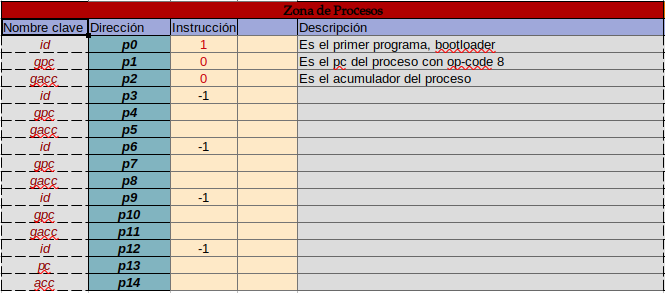
\includegraphics[scale=0.5]{media/Zona_procesos} 
		\caption{Representación de Zona de procesos}
		\label{fig:zprocesos}
	\end{figure}
	
	
	Ahora regresemos a la imagen \ref{fig:zprocesos},
	que aún tiene cosas que decirnos, ahora que ya entendemos como funcionan esas extrañas direcciones vemos que a la izquierda
	de la dirección hay una pequeña descripción para cada dirección y a la derecha una instrucción acompañada más a la derecha
	por una descripción, como vemos solo las primeras tres direcciones tienen una descripción y es que a partir de ahí el patrón
	se repite por que cada tres direcciones tenemos un nuevo proceso que empieza con un \textbf{id} y es acompañado por un 
	\textbf{gpc} y un \textbf{gacc} para guardar toda la información referente a un proceso, estos tres componentes están en
	direcciones contiguas para que el sistema operativo pueda ubicarlos a partir del \textbf{id} sino sería imposible. Otra cosa
	interesante a notar es que tenemos un proceso de ejemplo en las primeras tres direcciones, este proceso será importante más adelante,
	pero en las otras direcciones no hay nada salvo un $-1$ en cada dirección que contiene un \textbf{id}, esto es por que
	un $-1$ nos indica que no hay proceso ahí, y si no hay proceso ahí lo demás puede contener basura, no nos importa. Si lo noto
	no hay límite definido en la cantidad de procesos que se pueden guardar, pero cuando se lleve a la implementación
	ser definirá una cantidad que no debe ser muy grande.
	
	\subsection{Variables del sistema}

	Pasemos a las \textbf{variables del sistema}, podemos ver una representación de como sería esta región en la imagen 
	\ref{fig:varSis}, donde nos encontramos que las direcciones están representadas en lugar de por una $p$ inicial por una
	$c$ inicial haciendo referencia que en su mayoría son \textbf{constantes}, el funcionamiento es igual al de las
	direcciones mencionadas en las zonas de procesos, si se define $c=0050$ entonces $c5=c+5=0055$ sin mayor problema. Al igual
	que la zona de procesos la representación tiene a la izquierda de la dirección un nombre clave para esa dirección y a la derecha
	la instrucción y su descripción.
	
	
	\begin{figure}[h]
		\centering
		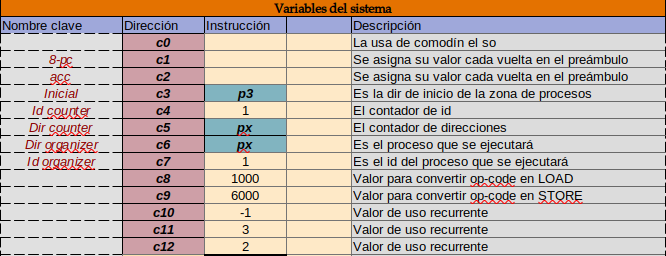
\includegraphics[scale=0.5]{media/Variables_Sistema} 
		\caption{Representación de Variables del sistema}
		\label{fig:varSis}
	\end{figure}
	
	Hay muchas cosas importantes aquí, empecemos por las direcciones $c1$ y $c2$; $c1$ guarda el valor
	de un acumulador sin más problemas y como se ve en su nombre clave $c1$
	guardara el valor de un  contador de programa o $pc$ con una ligera modificación,
	esta dirección guardará valores de contadores de programa pero
	con un \textbf{op-code} igual $8$, esto tiene sentido por que el valor de un $pc$ es una dirección, es decir un valor de tres
	dígitos en esta arquitectura, por lo que colocarle un código de operación en apariencia arbitrario no afecta en si
	el valor guardado. Si recordamos dijimos que cada \textbf{salto automático} del $pc$ se guarda ese valor en una dirección
	$e$, bueno es ese mismo valor el que modifica el \textbf{preámbulo} y manda a esta dirección con el código de operación $8$,
	el mismo preámbulo es el que manda el valor que se guarda en $c1$, así que en estas dos direcciones se encuentran los valores
	necesarios si es que se quiere actualizar los valores de un proceso.
	
	La siguiente que veremos es $c3$ que lleva por nombre clave \textit{Inicial}, esta guarda la dirección de inicio
	de la \textbf{Zona de procesos}, o bueno, algo así, lo que sucede es que como ya mencionamos el primer proceso es especial
	por lo que no le podemos considerar el inicio de la Zona de procesos. Esta variable es muy importante por que el
	sistema operativo necesitará una referencia de donde se encuentran sus procesos y cuando se vea el flujo de trabajo de este
	se entenderá mejor su importancia.
	
	Ahora veamos otro par de direcciones que vienen en equipo, $c4$ y $c5$, el \textbf{Id counter} y el \textbf{Dir counter} como
	lo dice su nombre clave. Este par de variables llevarán la cuenta de la cantidad de procesos que hay actualmente
	en la Zona de procesos, así como servir para la asignación de nuevos identificadores, por que si se agrega un nuevo proceso
	necesitamos saber cual es el último id usado y así asignar el siguiente a este nuevo proceso, eso nos lo dirá el
	\textbf{Id counter}, por otro lado esta bien que sepamos donde inician la zona de procesos, pero si vamos en
	el proceso 10 ¿donde guardaremos su identificador?, ahí es donde entra \textbf{Dir counter} que guarda la última dirección
	de la Zona de procesos utilizada para guardar un identificador de un proceso activo, así que basta con sumarle tres a ese
	valor para tener la siguiente dirección disponible para guardar un identificador. En $c5$ podemos ver la instrucción $px$, aunque
	aquí más bien es un número que representa una dirección pero es un poco lioso todo eso así que digámosle instrucción a todo
	lo que veamos en celdas de memoria y se harán las aclaraciones pertinentes cuando sea necesario, tal instrucción, como
	ya podrán intuir representa la dirección del identificador de un proceso por el prefijo $p$ ¿cual proceso? puede ser cualquiera
	y eso es lo que representa la $x$.
	
	Las siguientes dos variables están muy ligadas a las anteriores, $c6$ y $c7$, el \textbf{Dir organizer} y el \textbf{Id organizer},
	estas variables como su nombre lo indica organizan el lanzamiento, son las que dictan que proceso se va a lanzar. Es momento
	de especificar a que nos referimos con ``lanzar'' y como funcionará la \textbf{concurrencia} de CARDIAC v2, nos referimos
	a la acción de ``lanzar'' un proceso cuando iniciamos la ejecución de un proceso o la reanudamos si fue detenida en algún
	momento para permitir que el sistema operativo lanzará otro. El sistema operativo no tiene un mecanismo para priorizar
	el lanzamiento de procesos, por lo que solo los lanzará en lista, es decir si hay 5 procesos primero lanzará el número 2, este
	se pausará y el sistema operativo lanzará el 3, así hasta llegar al 5 y después de este el sistema revisará si hay un proceso
	adelante al verificar si el \textbf{Id counter} tiene un valor superior a 5, si no lo tiene quiere decir que no hay otro
	más y reinicia los lanzamientos con el proceso número 2. Pero ¿Que pasa con el proceso 1?, por fin diremos que tiene de especial
	este proceso.
	
	El primer proceso es el \textbf{bootloader} y es el socio principal(y único) del sistema operativo para administrar
	los proceso, al principio hablamos de que con el \textbf{bootstraping} podíamos lograr el arranque de la maquina y
	que el usuario cargara programas y los ejecutará únicamente ingresando instrucciones a CARDIAC, bueno, mantuvimos
	ese programa con el nombre de bootloader y el sistema operativo lo reconoce como el proceso 1. Este proceso para que
	sea realmente útil no debe ser interrumpido, en una maquina que soporte millones de ciclos por segundo esto no sería un
	problema, pero en CARDIAC v2 si lo es por que tu puedes tardar más de 20 ciclos en agregar un programa siguiendo las instrucciones
	de la sección de arranque y si el valor de $C$(los ciclos que tarda el pc en saltar) es menor a 20 te interrumpirá en tu tarea
	y esto no será cómodo para el usuario ni instructivo para ver los efectos de la concurrencia. Por ello la bandera de 
	\textbf{salto automático} no permitirá saltos si se esta ejecutando el sistema operativo o el proceso 1, más aún el
	sistema operativo no cederá el paso a otro programa si se esta ejecutando el proceso 1, por ello es que no se considera
	como un proceso igual a los demás ya que tiene un tratamiento especial. Hay dos formas de salir de este proceso, una es
	temporal, si terminas de añadir tu programa y das la instrucción de añadir programa a la zona de procesos se sale del proceso 1
	y se pasa al sistema operativo, la otra es con la instrucción $9000$, es decir mandar a borrar el proceso y por ende salir
	permanentemente de el, aunque hay una trampa aquí y es que es el único proceso que en realidad no se borra, más bien
	se bloquea. Si mandas a borrar el proceso 1 es por que ya terminaste de añadir tus programas, supongamos que añadiste 4 programas,
	entonces el sistema operativo bloquea el proceso 1 y empieza a ejecutar concurrentemente los otros cuatro programas, ahora
	proceso empezando por el proceso 2, cuando estos se terminen y se borren de la lista de procesos el \textbf{Id counter}
	regresará al valor de 1, indicando que ya no hay procesos a ejecutar y por lo tanto el sistema operativo desbloqueará el
	proceso 1 y lo lanzará para que puedas seguir añadiendo programas. Aún no se ha mencionado como ``añadir'' programas, por
	que si recuerda en la sección de arranque mencionamos que esa forma de ejecutar programas estaba incompleta y que se tenia
	que terminar de definir, eso se hará más adelante, pero era importante mencionarlo aquí por que es aquí donde
	se detalla el flujo de trabajo que usted tendrá al añadir programas.
	
	
	Las direcciones que quedan son $c0$ que es una dirección que usará el sistema operativo de comodín para guardar
	valores y recuperarlos, mientras que las demás son constantes, $c8$ y $c9$ servirán para cambiar los códigos de operación
	de una instrucción en particular, es decir si tenemos la instrucción $0050$ y queremos cargar en el acumulador lo que
	hay en la dirección $050$ le sumamos $c8$ a la instrucción para obtener $1050$, la instrucción para cargar el contenido
	de la dirección $050$, lo mismo sucede para $c9$ pero cuando queremos guardar algo en alguna dirección. En cuanto
	a $c10$, $c11$ y $c12$ están ahí por que se usan muy a menudo esos números y ahorra muchas lineas de código tenerlas mejor
	como constantes al alcance del sistema.
	
	
	\subsection{Preámbulo}
	
	Esta región es la encargada de dejar todo listo para que el sistema operativo funcione correctamente, como
	ya se menciono en la sección anterior es el que se encarga de mandar al contador de programa y el acumulador a
	sus zonas correspondientes. Pero vayamos por partes, primero como vemos en la imagen \ref{fig:preambulo} ahora
	tenemos las direcciones con una nomenclatura que sustituye la $c$ por la $e$ que representa a la región del preámbulo o
	exordio y funciona exactamente igual que las anteriores, solo que en este caso no se inicializa con $e0$ por que se menciona
	varias veces la dirección $e$ antes de este párrafo y podría llegar a ser confuso. Por otra parte notamos que
	el nombre clave aquí ya no es solo para una dirección sino para un grupo de estas y es que como se notará
	en el análisis de cada una, si bien tienen una función individual forman parte de una operación más grande y
	bien definida, esto sucede apenas aquí por que en realidad en las otras dos regiones no teníamos
	instrucciones como tal, sino números o datos a los que llamamos instrucciones para mantener la consistencia
	en el esquema, por que tanto en el esquema de preámbulo como el del sistema operativo central en la columna
	de instrucción hay instrucciones y datos por igual, esto no debe confundir al lector pues debe recordar que
	una instrucción lo será si el $pc$ la lee y el instruction register la interpreta aunque para nosotros
	sea un datos, por eso hay que ser cuidadosos de donde poner lo que para nosotros son datos.
	
	\begin{figure}[ht]
		\centering
		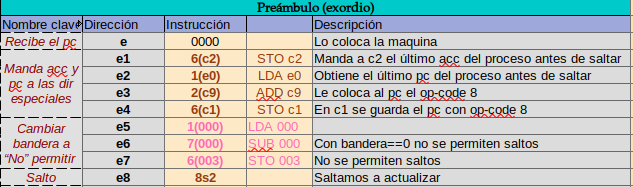
\includegraphics[scale=0.5]{media/Preambulo} 
		\caption{Representación del preámbulo}
		\label{fig:preambulo}
	\end{figure}
		
	Diseccionando lo que sucede
	en cada parte vemos que en efecto como se dijo antes $e$ recibe el $pc$ del proceso que se estaba ejecutando, pero
	nos falta algo para completar el proceso, el acumulador, este se consigue fácilmente en $e1$ con la instrucción que
	indica que se guarde en $c2$, pues el $pc$ salta directamente a $e1$ si la bandera se lo permite, por lo que en ese
	momento el acumulador no se ha tocado, esta intacto, podemos fácilmente guardarlo en $c2$ para que luego el sistema
	operativo actualice el valor del \textbf{gacc}(el acumulador guardado) con este valor. Después queda colocar el código
	de operación $8$ al valor del $pc$ almacenado en $e$ para mandarlo $c1$. Por último se activa la bandera que impide al 
	$pc$ saltar hacia $e1$ cada $C$ ciclos. Finalmente salta a $s2$, $s2$ como podrá intuir es la nomenclatura para el sistema
	operativo y se verá en la siguiente sección, pero antes hablemos sobre las formas de llegar a esta región, o más 
	bien la forma de llegar, por que cuando se borra un proceso o se añade no se pasa por el preámbulo, se va otra
	dirección que en su momento comentaremos, solo cuando el $pc$ realiza \textbf{saltos automáticos} llega aquí, y 
	¿cuando realiza salto automáticos? cuando se esta ejecutando cualquier proceso que no sea el 1 o el sistema operativo,
	así que viene aquí por que la única acción posible es actualizar ese proceso y lanzar otro, si el proceso se fuese a borrar
	o se añadiera un nuevo proceso se ``entra'' por otro lado al sistema operativo.
	
	
	% Cambiarlo por sistema minimo
	% Usar el diagrama y hacer más simple el diagrama
	\subsection{Sistema operativo central}
	
	Ahora si estamos en condiciones de hablar como funciona el sistema el sistema operativo central, la forma en que llamamos
	a la parte del sistema operativo que realiza las operaciones para la administración de tareas. En el diagrama que
	se puede observar en el anexo(la imagen anexada) vemos un diagrama de flujo del sistema operativo que servirá para explicar
	como funciona. Vamos a ver como es el flujo de trabajo con este sistema operativo, primero es el arranque con el 
	\textbf{bootstraping} que se carga con las instrucciones dadas al principio y este mismo se encargará de cargar todo el sistema
	operativo dentro de la memoria(todas las regiones) y una vez hecho eso el ahora \textbf{bootloader} estará listo
	para recibir instrucciones del usuario, instrucciones que podemos pensar como ``tarjetas'' que le puede mandar como
	entrada para \textbf{agregar un nuevo programa}, las instrucciones son como en la sección de \textbf{bootstraping}
	se detalla, van en pares, donde la primera es la dirección donde se guardara la siguiente instrucción o número a ingresar.
   Pero la forma de finalizar un programa será especial para que funcione la maquina con un sistema multitarea, podemos
   considerar como penúltimo par a la dirección del programa y la instrucción $9000$ para indicar que ahí acaba ese programa,
   pero después viene otro par que es para guardar la dirección de inicio de este nuevo programa en un lugar que el
   sistema operativo conoce, por lo que este último par es $0(s)$ seguido por la dirección de inicio del nuevo programa,
   donde $s$ es una dirección del sistema operativo central y de hecho ya se pueden imaginar que funciona
   como la nomenclatura para las otras regiones solo que con una letra nueva, es decir que si definimos en la implementación
   $s=100$ entonces $s20=s+20=120$. Si bien ese fue el último par aún falta una última instrucción, la de 
   \textbf{agregar un nuevo programa} que es $8(s55)$ y que se pone sola y al final, donde $s55$ es una dirección de memoria que
   sigue la idea de la nomenclatura mencionada, así
   si en la implementación se define $s=100$, entonces $s55==s+55=155$, y la por lo tanto la expresión $8(s55)=8155$, es decir
   ``salta a la dirección 155''. En la definición general se usaron unos paréntesis para evitar confusiones y dejar claro
   que $s55$ o $s$ son direcciones y lo que va antes del paréntesis es un \textbf{op-code}. En la implementación el usuario
   no se preocupara cuál es la dirección pues vendrá especificada la instrucción exacta para agregar el nuevo programa,
   así en el siguiente recuadro podemos ver un ejemplo de agregar un programa que recibe un número del usuario y le suma un uno
   y lo muestra:
   
   \begin{verbatim}
   	0200 Recibir datos
   	1200 Cargar dato
   	2001 Sumarle un uno
   	6200 Guardar dato
   	5200 Mostrar dato
   	9000 Terminar
   \end{verbatim}
   
   La forma en que el usuario cargaría este programa suponiendo que $s=100$
   sería con una tarjeta como la siguiente, que en la página le llaman \textbf{decir}:
   
   \begin{verbatim}
   	0300 En 300 cargar la primera instrucción
   	0200
   	
   	0301
   	1200
   	
   	0302
   	2001
   	
   	0303
   	6200
   	
   	0304
   	5200
   	
   	0305
   	9000
   	
   	0100 Guardar en s=100 la dirección de inicio del programa
   	0200 No importa el 0 por que se leerá como dirección
   	
   	8155 Saltar a 155 a agregar el nuevo programa
   	
   \end{verbatim}
   
   Como se puede apreciar al final se agrega la instrucción que agrega un nuevo programa al administrador de tareas, como tal
   no la agrega sino que salta al código que lo hará. Y es aquí donde vemos la primera ``entrada'' al sistema operativo,
   pues si se agrega un nuevo programa el contador de programa entra en los dominios del sistema operativo, esto se puede
   ver en la parte central del diagrama donde con un color rojo de fondo esta la entrada que dice que se agrego
   un nuevo programa, aunque primero se valida si en realidad hay una dirección donde el sistema la espera, después el sistema
   agrega el programa como se muestra en la parte del diagrama con fondo morado para finalmente salir y llegar 
   a un rombo de decisión donde pregunta si el \textit{Id organizer} es igual a uno, esta pregunta significa que
   si se estaba ejecutando el proceso 1, el \textbf{bootloader} y naturalmente en una ejecución normal así lo es
   por lo que salta directamente de regreso al bootloader sin hacer más preguntas el sistema operativo, pero esto ¿por que
   lo hace? por que es la mejor manera de mostrar la concurrencia de procesos, pues la idea es primero agregar
   los programas que se deseen, de forma que el administrador de tareas ya los tendrá contemplados y al final
   si hay no hay más procesos que agregar y se este ejecutando el bootloader el usuario ingrese $9000$ lo que
   bloqueará el proceso 1 y pasará a ejecutar todos los procesos que tiene pendientes, cuando terminen de ejecutarlos
   pasará se volverá a activar el bootloader.
   
   
   Ya vimos una de las entradas al sistema operativo, la otra como es normal pensar es la de \textbf{borrar programa},
   que como ya vimos si se ejecuta la instrucción $9000$ que nos dice que saltará a la dirección \textbf{B}, ahora que
   ya tenemos un poco más de idea sobre la nomenclatura para facilitar la identificación de regiones
   de código la podemos sustituir con la dirección $s14$ que nos deja claro que con la instrucción de borrar programa
   se llega directamente a la región del sistema operativo central. En el diagrama todo el proceso del borrado se muestra
   con un color azul de fondo para el borrado de procesos comunes y de azul claro para el ``borrar'' del proceso 1, en
   ambos casos terminamos preguntando si el \textbf{Id counter} es igual a 1, pregunta que también se hace si se ha entrado
   desde \textbf{agregar nuevo programa}, pero en ese caso no tiene mucho sentido y esta ahí más bien para no afectar el
   flujo de ejecución de instrucciones. Y es que lo que significa la pregunta es que si el \textit{Id counter} es igual
   a uno quiere decir que ya no hay procesos a ejecutar por lo que es necesario activar nuevamente el bootloader
   y ya no hacer más preguntas, en caso de que el \textit{Id counter} sea distinto de uno quiere decir que hay al menos un
   proceso que aún no se ha terminado, pues como veremos un poco más adelante si un proceso se borra el \textit{Id coutner}
   disminuye su valor, siempre que no sea el proceso especial, por ende si acaba de agregar un proceso el \textit{Id counter}
   inevitablemente es mayor a uno.
   
   Pero ¿y que pasa cuando se borra un proceso de los normales? bueno, es el momento idóneo para explicar como 
   funcionan los procesos en este sistema. Como vimos los procesos tienen identificadores empezando por el número 2
   y la forma en que el \textit{Id organizer} decide cuál será ejecutado es simplemente por orden y cuando se ha lanzado el
   último se regresa al primero, esto significa que el organizador no contempla que si hay 5 procesos el proceso con identificador
   4 no exista por que fue borrado, por lo que en este sistema los procesos \textbf{no tienen un id inmutable}, este id cambiara
   si es necesario. Supongamos que hay $n$ procesos y borramos el proceso $k$ con $id=5$, tenemos que revisar si hay proceso $k+1$
   con forzosamente $id=6$ pues son consecutivos,
   $k+2$ con $id=7$ y así sucesivamente, si los hay lo que haremos es mover la información del proceso $k+1$ a donde se encuentra
   información de $k$, todo menos el id, de forma que ahora en la zona de procesos en la parte que corresponde al $id=5$
   estará la información de $k+1$, y ahora se quedará borrar el proceso con $id=6$ de la misma forma que se
   hizo antes se verificará si hay un proceso siguiente, esto se hará de forma iterativa hasta que no haya más procesos adelante
   y entonces simplemente el último $id$ tomará el valor de -1 indicando que no hay proceso ahí, el \textit{Id counter}
   disminuirá su valor en uno y el \textit{Dir counter} disminuirá su valor en tres, pues el último proceso
   está tres direcciones antes.
   
   Para que quede más clara la idea podemos pensar en la Zona de proceso de la imagen \ref{fig:procesos1},
   donde hay cuatro procesos activos con su respectiva información, si decidiéramos eliminar el número
   3 o más bien este se terminará lo que pasaría es lo que se ve en la imagen \ref{fig:procesos2}, se
   recorren la información de los procesos 4 y 5, y el que se elimina en realidad es el número 5 que
   toma el valor de -1, y como se puede notar queda información remanente en la parte del proceso 5,
   pero no importa por que si está con un -1 no se considera un proceso.
   
   \begin{figure}
		  	\centering
		  			\begin{subfigure}[b]{0.48\textwidth}
				      \centering
						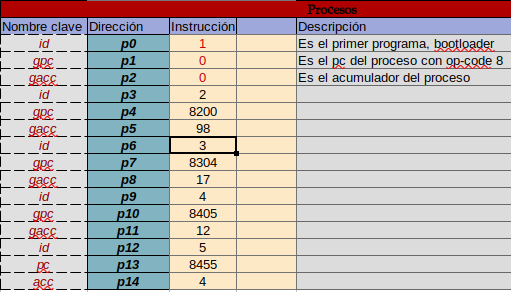
\includegraphics[width=\textwidth]{media/procesos1} 
						\caption{Cuatro procesos activos}
						\label{fig:procesos1}
				  \end{subfigure}
			\hfill
				  \begin{subfigure}[b]{0.48\textwidth}
				      \centering
						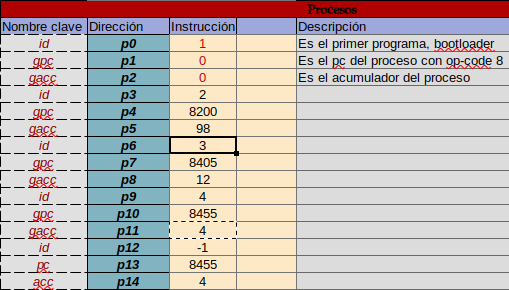
\includegraphics[width=\textwidth]{media/procesos2} 
						\caption{Tres procesos activos}
						\label{fig:procesos2}
				  \end{subfigure}
		   \caption{Ejemplo de Zona de procesos}
		   \label{fig:ejemploZona}
	\end{figure}

	
	Esto que podría parecer que dificulta las cosas en realidad las facilita, pues así el \textbf{Id organizer} no
	tiene que estar preguntando si el proceso 3 existe o no y la forma de acceder a la memoria de la zona de procesos
	es siempre ir agregando procesos adelante del último, por lo que no hay que hacer búsquedas lineales para encontrar
	un lugar libre o desperdiciar memoria.
	
	
	
	Finalmente queda una entrada, a de \textbf{actualizar}, a esta se llega por el preámbulo cada que el $pc$ salta
	de forma automática y en el diagrama esta de color café el preámbulo y en verde la actualización. Como
	el preámbulo ha preparado todo el sistema operativo solo tiene que actualizar los valores del $gpc$ y del
	$gacc$ para el proceso que se estaba ejecutando, esto es sumamente fácil por que esos valores ya están en la región
	de variables del sistema y por que cada que se lanza un proceso se guarda en $s1$ la dirección donde
	se encuentra el $id$ con \textbf{op-code} 6
   del proceso que se ha lanzado y por ende toda la información de este, así cuando se borra un proceso
	o se actualiza solo basta con buscar en $s1$ para saber de cuál proceso se trata. El por que se tiene ese código
	de operación en especial es por que facilita el funcionamiento del sistema, si se quiere ver en detalle el
	funcionamiento el código se encuentra en el anexo también, pero diremos que con el código de operación 6 si se
	le suma un uno estaríamos diciendo que guarde un valor en la dirección siguiente al $id$ que es la
	dirección donde se guarda el $gpc$ de ese proceso, he ahí el por que es practico tenerlo. Una vez que se ha
	actualizado llegamos a la parte naranja en la que todas las entradas confluyen, siempre que no se este ejecutando
	el proceso 1 o que por el contrario y a no hay procesos a ejecutar, y podemos llamarle a esta área el \textbf{área de lanzamiento},
	pues es aquí donde se decide cuál proceso será lanzado. Se empieza por aumentar el \textbf{Id organizer} y verificar
	si no se ha pasado ya del máximo de procesos activos, si lo ha hecho se reinicia y justo antes de
	lanzar el proceso la bandera de \textbf{salto automático} se cambia a permitir saltos. Si bien no se ha comentado aquí
	el \textbf{Dir organizador} y el \textbf{Dir counter} aumentan y disminuyen con sus respectivos \textbf{Id organizer}
	y \textbf{Id counter}, estos y más detalles del funcionamiento del sistema operativo están más claros en el diagrama que
	se debe leer acompañado de esta explicación, si se quiere ver a detalle profundo el funcionamiento
	del sistema operativo véase el anexo.
	
	
	\clearpage	
	\newpage
	\selectlanguage{spanish}
		\bibliography{CARDIAC}
	\selectlanguage{spanish}
		\bibliographystyle{apacite}
	
	

\end{document}
